
One often needs the strain rate tensor in geodynamics for two main reasons:
1) it is a quantity which 'helps' with interpreting results
2) it is needed in the non-linear rheology, typically power-law.

Let us assume the scalar nodal field $f$ (e.g., temperature, 
components of velocity, ...) has been obtained by solving a FE problem.
Anywhere within an element 
the given finite element solution 
\[
f^h(x,y)=\sum_k N_k(x,y) f_k
\]
 
We wish to compute the field $\vec g^h = \vec \nabla f^h$ on the nodes 
with the highest accuracy. 

For any point inside an element, this problem is trivial and we have 
\begin{equation}
\vec g^h(x,y) = \sum_{k=1}^m \vec\nabla N_k (x,y) f_k \label{eq:derr1}
\end{equation}
This method works adequately everywhere inside the element, but 
since the basis functions derivatives
are not uniquely defined on the nodes 
this problem requires careful attention
to arrive at the best result.

\begin{center}
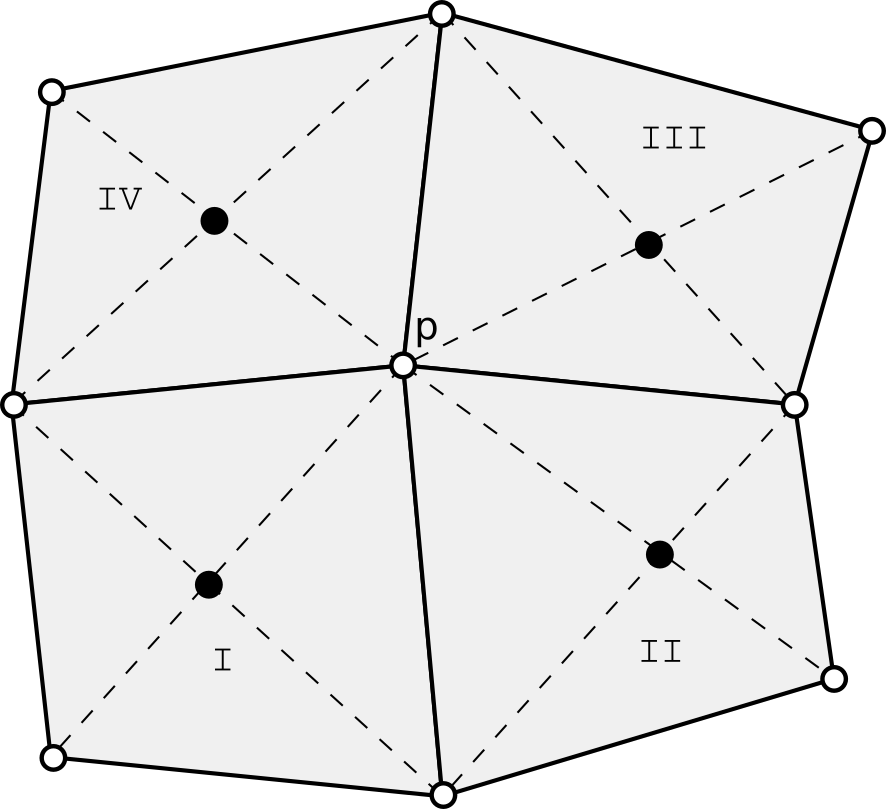
\includegraphics[width=7cm]{images/patch/patch3}
\end{center}

%____________________________________________________
\subsubsection{Centroid-to-node method ("method 1")}
In this case the gradient is first computed in the 4-element patch 
to which node $p$ belongs to as shown in Fig. (\ref{fig:patches}).
The gradient $\vec g$ is computed at the centroid of each element of the 
patch and averaged out to yield $\vec g_p$.

\[
\bm g_p^h = \frac{1}{4} \sum_{e} \left( \sum_{k=1}^m  (\vec\nabla N_k f_k)_{\bm r=\bm r_c} \right)_e
\]
where $\bm r_c$ stands for the location of the centroid. 

This technique is similar to the one of pressure smoothing showcased 
in Braun \etal (2008) \cite{brtf08}
and is mentioned on p. 865 of Gresho \& Sani \cite{grsa}.

Although very simple to implement, this approach is not without problem since 
the algorithm cannot be applied to the nodes on the boundary and an ad-hoc 
rule muct be adopted for these. 


%____________________________________________________
\subsubsection{Corner-to-node method ("method 2")}

For each element of the patch the value of $\vec g$ is computed at node $p$ and the obtained
values are then averaged out. At the time of writing, this is the technique implemented in  
ASPECT.
\[
\bm g_p^h = \frac{1}{4} \sum_{e} \left( \sum_{k=1}^m  (\vec\nabla N_k f_k)_{\bm r=\bm r_p} \right)_e
\]


%________________________________________________________
\subsubsection{Consistent approach using basis functions ("method 3")}

What follows is formulated in 2D Cartesian coordinates for simplicity. 
Let us start from the function $g$ which is the gradient of the function $f$
in the $x$-direction:
\[
g(x,y) = \frac{\partial f}{\partial x}(x,y)
\]
If we left-multiply this equation by a basis function $N_i(x,y)$ 
and integrate over an element, we arrive at 
\begin{equation}
\int_{\Omega_e} N_i(x,y)\; g(x,y)\; dV =
\int_{\Omega_e} N_i(x,y)\; \frac{\partial f}{\partial x}(x,y)\; dV
\label{eq:derr2}
\end{equation}
The function $g$ is represented inside an element by
\[
g^h(x,y) = \sum_j N_j(x,y) g_j = \vec{N} \cdot \vec{g}
\]
where $\vec{g}=(g_1,g_2,\dots g_{m_v})$ is the vector of nodal values for the element
and $\vec{N}$ is the vector of basis functions.
Likewise we have:
\[
\left. \frac{\partial f}{\partial x}(x,y) \right|^h = \frac{\partial \vec{N}}{\partial x}\cdot \vec{f}
\]
where $\vec{f}=(f_1,f_2,\dots f_{m_v})$ is the vector of $f$ nodal values for the element.
When we write \eqref{eq:derr2} for $i=1,2,...m_V$ we arrive at
\[
{\bm M}\cdot \vec{g} = {\bm G}_x\cdot \vec{f}
\]
where ${\bm M}$ is the elemental mass matrix:
\[
{\bm M}=\int_{\Omega_e} \vec{N}^T \vec{N} dV
\]
and ${\bm G}_x$ is the gradient matrix 
\[
{\bm G}_x=\int_{\Omega_e} \vec{N}^T \frac{\partial \vec{N}}{\partial x} dV
\]
Both matrices are of size $m_v \times m_v$.
After the assembly process we are now ready to solve the global system and obtain
the derived nodal value at all nodes. 
This method is particularly interesting because it can use the existing algorithms 
already present in any FE which has solved the PDE to obtain $f$.  

The nodal strain rate components are obtained as follows:
\begin{eqnarray}
\dot{\varepsilon}_{xx} &=& {\bm M}^{-1} \cdot {\bm G}_x \cdot \vec{U} \\
\dot{\varepsilon}_{yy} &=& {\bm M}^{-1} \cdot {\bm G}_y \cdot \vec{V} \\
\dot{\varepsilon}_{xy} &=& \frac{1}{2} {\bm M}^{-1} \cdot \left( {\bm G}_x \cdot \vec{V} + {\bm G}_y \cdot \vec{U} \right)
\end{eqnarray}
where $\vec{U}$ is the vector of all nodal $u$ and $\vec{V}$ is the vector of all nodal $v$.


idea: try lumping M?

make link with consistent pressure recov for q1p0








